\documentclass{article}
\usepackage{mathtools}
\usepackage{amssymb}
\usepackage{amsthm}
\usepackage{extarrows}
\usepackage{graphicx}
\usepackage{subcaption}
\usepackage{enumitem}
\title{Assignment 6}
\date{October 17, 2020}
\author{Haixiang Zhu}
\begin{document}
\maketitle
    \begin{enumerate}
        \item Numerical Solution (See the attached file ``ps6\_q1.m'')
        \begin{enumerate}
            \item Discretize the state space
            \item Denote $V_1(k)$
            \item Solve the maximization problem that defines $V_2(k),g_2(k)$
            \item Plot $g_2(k)$
            \begin{figure}[h!]
                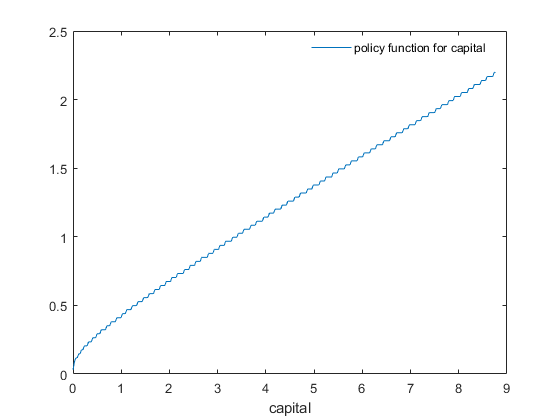
\includegraphics[width=\linewidth]{6_1d.png}
                \caption{$g_2(k)$, with N=300}
            \end{figure}
            \item Plot $V_1(k),V_2(k)$
            \clearpage
            \begin{figure}[h!]
                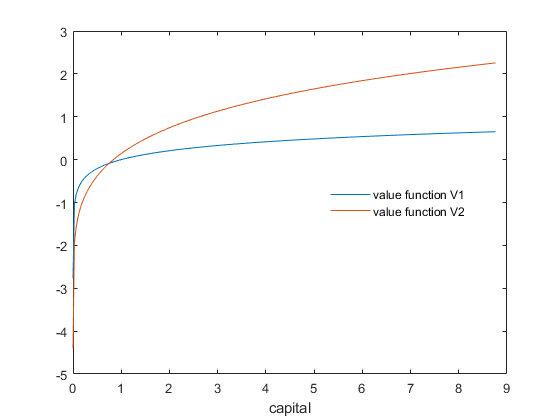
\includegraphics[width=\linewidth]{6_1e.png}
                \caption{$V_1(k)$ and $V_2(k)$, with N=300}
            \end{figure}
            $V_1(k)$ and $V_2(k)$ are different because the value function $V_1(k)$ is not true. The two functions would coincide under the right guess.
            \item Compute $V_3(k),g_3(k)$
            \item Plot $V_1(k),V_2(k),V_3(k)$
            \begin{figure}[h!]
                \begin{subfigure}[b]{.55\linewidth}
                    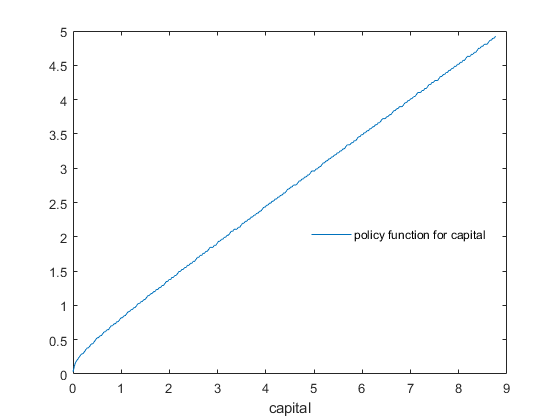
\includegraphics[width=\linewidth]{6_1f.png}
                    \caption{$g_3(k)$,with N=300}
                \end{subfigure}
                \begin{subfigure}[b]{.55\linewidth}
                    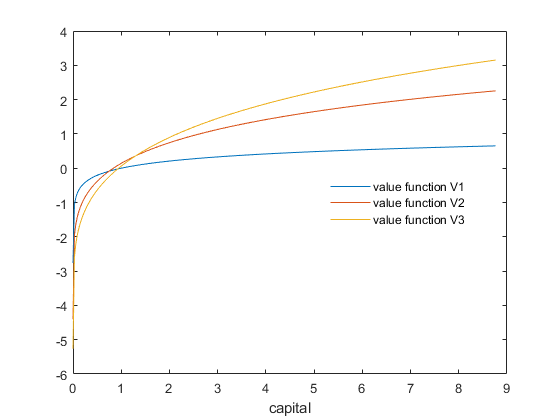
\includegraphics[width=\linewidth]{6_1g.png}
                    \caption{$V_1(k)$, $V_2(k)$ and $V_3(k)$, with N=300}
                \end{subfigure}
                \caption{Value and policy functions}
            \end{figure}
        \end{enumerate}
        \item Iteration (See the attached file ``ps6\_q23.m'')
        \begin{enumerate}
            \item The Bellman equation
            \begin{align*}
                &V(k)\enspace=\max_{c,k'}\{\ln(c)+\beta V(k')\}\\
                &\begin{array}{r@{\quad}l}
                    s.t.&c+k'-(1-\delta)k=k^\alpha\\
                    &c\ge0\\
                    &k'\ge0\\
                    &k\enspace given    
                \end{array}           
            \end{align*}
        \end{enumerate}
        \begin{figure}[h!]
                \begin{subfigure}[a]{.55\linewidth}
                    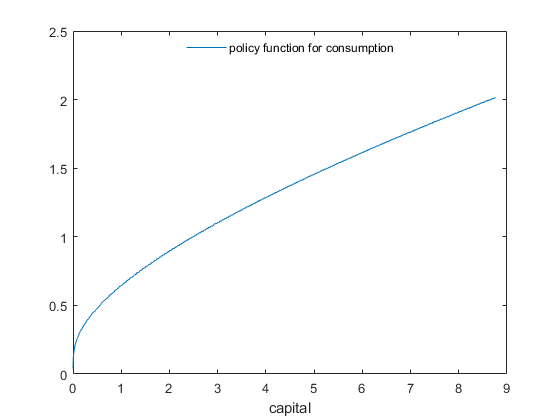
\includegraphics[width=\linewidth]{6_2a2.png}
                    \caption{$g^c(k)$, with N=1200}
                \end{subfigure}
                \begin{subfigure}[a]{.55\linewidth}
                    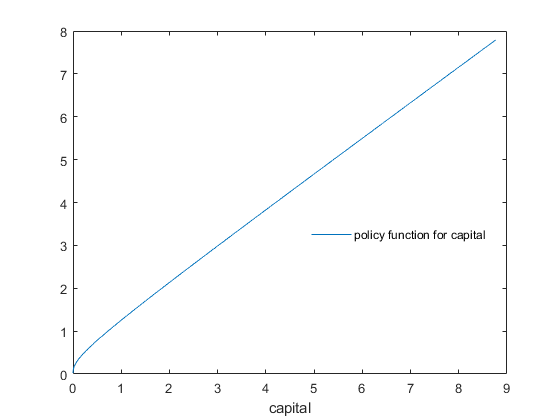
\includegraphics[width=\linewidth]{6_2a3.png}
                    \caption{$g^k(k)$, with N=1200}
                \end{subfigure}
            \begin{center}
                \begin{subfigure}[b]{0.7\linewidth}
                    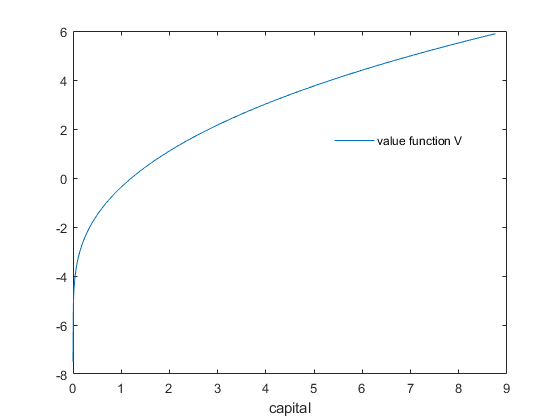
\includegraphics[width=\linewidth]{6_2a1.png}
                    \caption{$V(k)$, with N=1200}
                \end{subfigure}
            \end{center}
            \caption{Value and policy functions}
        \end{figure}
        \clearpage
        \item Simulation
        \begin{enumerate}
            \item Plot consumption, investment and output
            \begin{figure}[h!]
                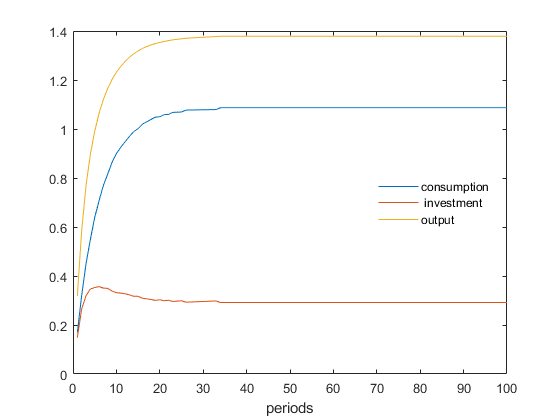
\includegraphics[width=\linewidth]{6_3a.png}
                \caption{Simulation, with periods=100}
            \end{figure}
            \item Difference between solution and simulation\\
            Solution includes functional approach and numerical one, which can both create simulation and be considered continuous.
            The latter one is limited by the length of input while the former is not.\\
            Simulation is discrete and belongs to sequence problem, the major elements of which is initial value and how to transit from current state to next state like probability transition matrix.
            Sometimes, simulation can be converted into functional one.
        \end{enumerate}
    \end{enumerate}
\end{document}